% \documentclass[handout, xcolor=table]{beamer}
\documentclass[xcolor=table]{beamer}

%-----------------------[ Macros ]----------------------------------------------%

%-----------------------[ Packages ]-------------------------------------------%

\usepackage[utf8]{inputenc}
\usepackage[brazilian]{babel}
% \usepackage[english]{babel}
\usepackage[T1]{fontenc}
\usepackage{lmodern}
\usepackage{amsfonts}
\usepackage{indentfirst}
\usepackage{xspace}
\usepackage{setspace}
\usepackage{geometry}
\usepackage{mathtools}
\usepackage{amsmath}
\usepackage{amsthm}
\usepackage{subcaption}
\usepackage{pdfpages}
\usepackage{hanging}
\usepackage{pdfpages}
\usepackage{nicefrac}
\usepackage{graphicx}
\usepackage[labelformat=empty]{caption}
\usepackage{booktabs, multirow} % for borders and merged ranges
% \usepackage[hyperpageref]{backref}
% \usepackage[
%   scr=boondox, % heavily sloped
%   cal=esstix % slightly sloped
% ]{mathalpha}
\usepackage{xmpmulti}
\usepackage{appendixnumberbeamer}

% Tikz:
\usepackage{tikz}
% \usetikzlibrary{ipe} % ipe compatibility library
\usetikzlibrary{calc, arrows, arrows.meta, patterns}

%-----------------------[ Colors ]---------------------------------------------%

\definecolor{red}{rgb}{1,0,0}
\definecolor{blue}{rgb}{0,0,1}
\definecolor{green}{rgb}{0,1,0}
\definecolor{yellow}{rgb}{1,1,0}
\definecolor{orange}{rgb}{1,0.647,0}
\definecolor{gold}{rgb}{1,0.843,0}
\definecolor{purple}{rgb}{0.627,0.125,0.941}
\definecolor{gray}{rgb}{0.745,0.745,0.745}
\definecolor{brown}{rgb}{0.647,0.165,0.165}
\definecolor{navy}{rgb}{0,0,0.502}
\definecolor{pink}{rgb}{1,0.753,0.796}
\definecolor{seagreen}{rgb}{0.18,0.545,0.341}
\definecolor{turquoise}{rgb}{0.251,0.878,0.816}
\definecolor{violet}{rgb}{0.933,0.51,0.933}
\definecolor{darkblue}{rgb}{0,0,0.545}
\definecolor{darkcyan}{rgb}{0,0.545,0.545}
\definecolor{darkgray}{rgb}{0.663,0.663,0.663}
\definecolor{darkgreen}{rgb}{0,0.392,0}
\definecolor{darkmagenta}{rgb}{0.545,0,0.545}
\definecolor{darkorange}{rgb}{1,0.549,0}
\definecolor{darkred}{rgb}{0.545,0,0}
\definecolor{lightblue}{rgb}{0.678,0.847,0.902}
\definecolor{lightcyan}{rgb}{0.878,1,1}
\definecolor{lightgray}{rgb}{0.827,0.827,0.827}
\definecolor{lightgreen}{rgb}{0.565,0.933,0.565}
\definecolor{lightyellow}{rgb}{1,1,0.878}
\definecolor{black}{rgb}{0,0,0}
\definecolor{white}{rgb}{1,1,1}

%-----------------------[ Commands ]-------------------------------------------%

\newcommand\mycomment[1]{} % block comment

\newcommand{\FPT}{\ensuremath{\mathcal{F}\mathcal{P}\mathcal{T}}\xspace}
\newcommand{\XP}{\ensuremath{\mathsf{XP}}\xspace}
\newcommand{\PP}{\ensuremath{\mathrm{P}}\xspace}
\newcommand{\NP}{\ensuremath{\mathrm{NP}}\xspace}

\newcommand{\dist}{\text{dist}}
\newcommand{\cost}{\text{cost}}
\newcommand{\opt}{\text{OPT}}
\newcommand{\makespan}{\emph{makespan}}

\newcommand{\cala}{\mathcal{A}}
\newcommand{\calb}{\mathcal{B}}
\newcommand{\cali}{\mathcal{I}}
\newcommand{\call}{\mathcal{L}}
\newcommand{\calo}{\mathcal{O}}
\newcommand{\cals}{\mathcal{S}}
\newcommand{\calt}{\mathcal{T}}

\newcommand{\R}{\rm I\!R}
\newcommand{\N}{\rm I\!N}
\newcommand{\overeps}{\nicefrac{1}{\varepsilon}}
\newcommand{\B}{$\bullet$}

\newcommand\rest[2]{\left.{#1}\right|_{#2}} % function restriction

\DeclarePairedDelimiter\ceil{\lceil}{\rceil}
\DeclarePairedDelimiter\floor{\lfloor}{\rfloor}
\DeclareMathOperator*{\argmax}{arg\,max}
\DeclareMathOperator*{\argmin}{arg\,min}

%-----------------------[ Proof Environments ]---------------------------------%

% \newtheorem{definition}{Definição}
\newtheorem{thm}{Teorema}
\newtheorem{cor}{Corolário}
\newtheorem{conj}{Conjectura}
\newtheorem{lem}{Lema}
\newtheorem{obs}{Observação}


\newcounter{finalframe}
\newcommand{\stopcounter}{
  \setcounter{finalframe}{\insertframenumber}
}

\newcommand{\resumecounter}{
  \setcounter{framenumber}{\value{finalframe}}
}

\newcommand{\inccounter}{
  \setcounter{framenumber}{\value{finalframe} + 1}
}

%-----------------------[ Template ]-------------------------------------------%

\mode<presentation> {
    \usetheme[sectionpage=none, progressbar=frametitle, block=fill]{moloch} % modern fork of the metropolis theme
    \setbeamertemplate{footline}[frame number] % to replace the footer line in all slides with a simple slide count
}
\setbeamerfont{footnote}{size=\tiny}
\setbeamertemplate{navigation symbols}{}
\setbeamertemplate{footnote}{%
    \hangpara{2em}{1}%
    \makebox[2em][l]{\tiny\insertfootnotemark}%
    \hspace{-1em}\tiny\insertfootnotetext\par\vspace{0.2cm}%
}
\setbeamercolor{background canvas}{bg=white}

%-----------------------[ (Sub)Section Slides ]--------------------------------%

\AtBeginSection[]{
    \begin{frame}[plain,noframenumbering]
        \setbeamercolor{title}{bg=mDarkTeal,fg=black!2}
        \vfill
        \centering
        \begin{beamercolorbox}[sep=8pt,center,shadow=true]{title}
            \usebeamerfont{title}\insertsectionhead\par%
        \end{beamercolorbox}
        \vfill
    \end{frame}
}

% \makeatletter
% \newcommand{\subseqslide}{
% \begin{frame}
%   \setbeamercolor{title}{bg=mDarkTeal,fg=black!2}
%   \centering
%   \begin{minipage}{22em}
%     \raggedright
%     \begin{beamercolorbox}[sep=8pt,center,shadow=true]{title}
%         \usebeamerfont{title}\insertsectionhead\par%
%     \end{beamercolorbox}
%     \usebeamertemplate*{progress bar in section page}
%     \par
%     \ifx\insertsubsectionhead\@empty\else%
%       \vskip-.6\baselineskip
%       \usebeamercolor[fg]{subsection title}%
%       \usebeamerfont{subsection title}%
%       \insertsubsectionhead{}
%     \fi
%   \end{minipage}
%   \par
%   \vspace{\baselineskip}
% \end{frame}
% }

% \AtBeginSubsection[]{%
% \subseqslide

% \setcounter{tocdepth}{3}
% \frame<beamer>{ 
%   \frametitle{}
%   \centering
%   \begin{minipage}{20em}
%   \tableofcontents[
%     currentsection,currentsubsection,sectionstyle=show/hide,subsectionstyle=show/shaded/hide,subsubsectionstyle=show/show/hide/hide
%   ]    
%   \end{minipage}
  
% }
% }
% \makeatother

%-----------------------[ Title page ]-----------------------------------------%

\renewcommand*{\thefootnote}{\arabic{footnote}}
\title{
  \large{An XP Approximation Scheme for AFTP in 2D}%
  \texorpdfstring{\footnote{
    Supported by the São Paulo Research Foundation~(FAPESP) grant
    %
    \mbox{2023/12529-8}
    %
    and by the National Council for Scientific and Technological Development~(CNPq) grants
    %
    \mbox{\#312271/2023-9},  % pq leh
    \mbox{\#404315/2023-2}.  % univ fkm
    }}{}
}

\titlegraphic{
  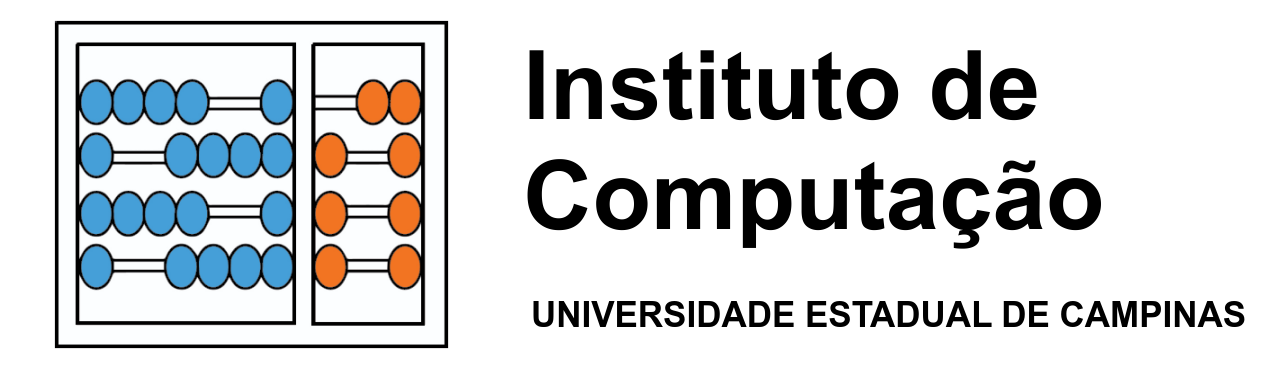
\includegraphics[height=1.cm]{logos/ic.png}
  \hfill
  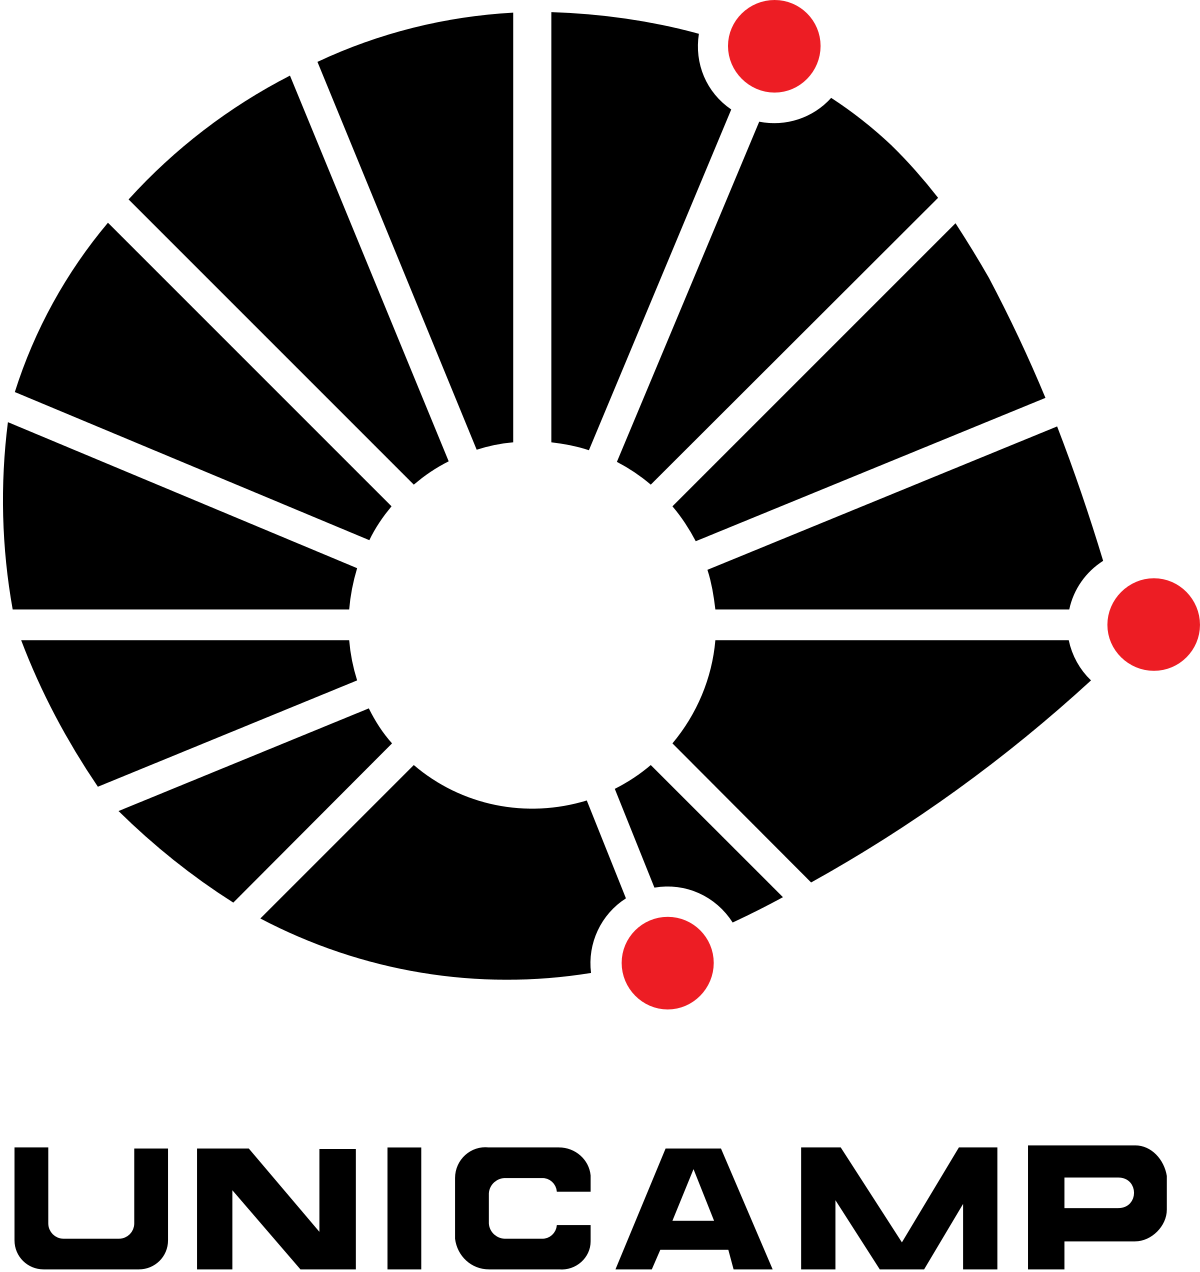
\includegraphics[height=1.2cm]{logos/unicamp.png}
}

\author{
  \textbf{Lucas de Oliveira Silva}\texorpdfstring{\\}{}
  Lehilton Lelis Chaves Pedrosa
}

\institute{Instituto de Computação, Unicamp}

\date{23rd of July, 2025}

\begin{document}

\begin{frame}[plain]
  \titlepage
\end{frame}

% \setcounter{tocdepth}{2}
% \begin{frame}{Sumário}
%   \tableofcontents
% \end{frame}

%------------------------------------------------------------------------------%

\section{Freeze-Tag Problem Original}
\stopcounter
\begin{frame}{Origem}
  O \textbf{Freeze-Tag Problem (FTP)} surge como um problema de robótica de enxame em 2002~\cite{Arkin02}:
  \bigbreak
  \begin{minipage}{\linewidth}
    \centering
    \multiinclude[format=png, start=0, end=4, graphics={height=5cm}]{FTP/ftp_example/Temp}
  \end{minipage}
\end{frame}
\inccounter

\begin{frame}{Alguns Resultados}
  \begin{thm}[Arkin et al.~\cite{Arkin02}]
    Existe um EPTAS para o FTP com distâncias $L_p$ em qualquer espaço de dimensão fixa $\R^d$.
    \pause
    
    \medskip
    O tempo de execução é $O(n \log n) + 2^{O(d(\overeps)^d\log{(\overeps)})}$.
  \end{thm}
\end{frame}

\begin{frame}{Alguns Resultados}
  \begin{thm}[Abel et al.~\cite{Yu17}]
    O FTP é NP-difícil para distância $L_2$ no plano.
  \end{thm}

  \pause
  \begin{thm}[Demaine e Rudoy~\cite{Erik17}]
    O FTP é NP-difícil para distâncias $L_p$, onde $p>1$, em 3D.
  \end{thm}

  \pause
  \begin{thm}[Pedrosa e Silva~\cite{Lu23}]
    O FTP é fortemente NP-difícil para distância $L_1$ em 3D.
  \end{thm}
\end{frame}


\section{Angular Freeze-Tag Problem}
%------------------------------------------------------------------------------%

\stopcounter
\begin{frame}{Origem}
  O \textbf{Angular Freeze-Tag Problem} surge como um problema de \textbf{\emph{broadcast}} entre satélites em 2018~\cite{Fe18}:
  \bigbreak
  \begin{minipage}{\linewidth}
    \centering
    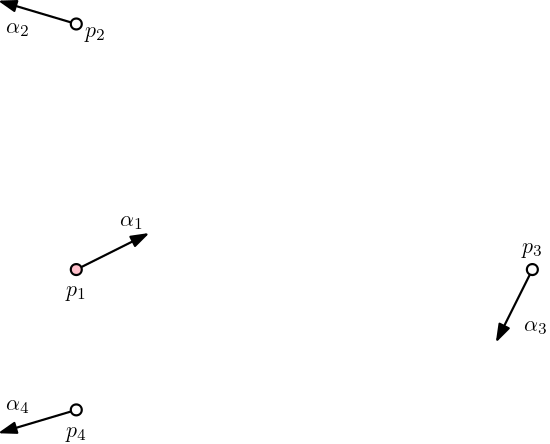
\includegraphics[height=4cm]{AFTP/instance/Temp-0.png}
  \end{minipage}
\end{frame}
\inccounter

\begin{frame}{Motivação}
  \begin{itemize}[<+->]
    \item Dado o crescimento das constelações de satélites, precisamos de estrategias de transmissão eficientes;
    
    \item Recursos limitados restringem a movimentação dos satélites;

    \item Grandes distâncias impossibilitam um \emph{broadcast} simultâneo.
  \end{itemize}
\end{frame}

\begin{frame}{Instância}
  \begin{itemize}[<+->]
    \item Assumimos um \textbf{enxame uniforme};

    \item Conjunto $P = \{p_1, \dots, p_n\}\subseteq \R^2$ de \textbf{posições distintas};

    \item Cada $p_i$ está associado a um satélite com \textbf{ângulo inicial} $\alpha_i$;

    \item Inicialmente, apenas $p_1$ contém \textbf{um dado} a ser propagado;

    \item Apenas os satélites que já receberam o dado podem ajustar suas antenas.
  \end{itemize}
\end{frame}

\begin{frame}{Solução}
  \centering
  \textbf{Rotações} a serem seguidas \textbf{após o recebimento} do dado:

  \pause

  \bigskip
  \begin{minipage}{\linewidth}
    \centering
    \colorbox{white}{\multiinclude[format=png, start=0, end=3, graphics={height=5.5cm}]{AFTP/instance/Temp}}
  \end{minipage}
\end{frame}

\begin{frame}{Definição mais Formal}
  \begin{itemize}[<+->]
    \item \textbf{Conjunto de cronogramas} $S$;

    \item O cronograma de cada satélite $p_i\in P$ é composto por uma \textbf{direção inicial} $d_i$ \pause e uma \textbf{sequência de ângulos} $S_i=(s_{i,1}, \dots, s_{i,k_i})$.
  \end{itemize}
\end{frame}

\begin{frame}{Exemplo}
  \begin{minipage}{\linewidth}
    \centering
    \colorbox{white}{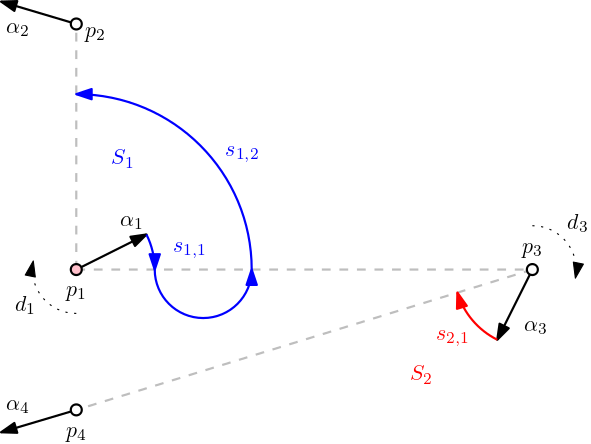
\includegraphics[height=5.5cm]{AFTP/solution.png}}
  \end{minipage}
\end{frame}

\begin{frame}{Dois Objetivos}
  \begin{itemize}[<+->]
    \item O \textbf{makespan ($\mathbf{M(S)}$)} de uma solução $\mathbf{S}$ é o instante em que o último satélite recebe o dado (\textbf{AFTP});
    
    \item A \textbf{energia total ($\mathbf{E(S)}$)} é a soma de todas as rotações realizadas por todos os agentes (\textbf{E-AFTP});
    \bigbreak

    \item Note que $E(S) \ge M(S)$.
  \end{itemize}
\end{frame}

\begin{frame}{Comparação}
  \centering
  Seja $\varepsilon < \theta$:

  \bigskip
  \begin{minipage}{\linewidth}
    \centering
    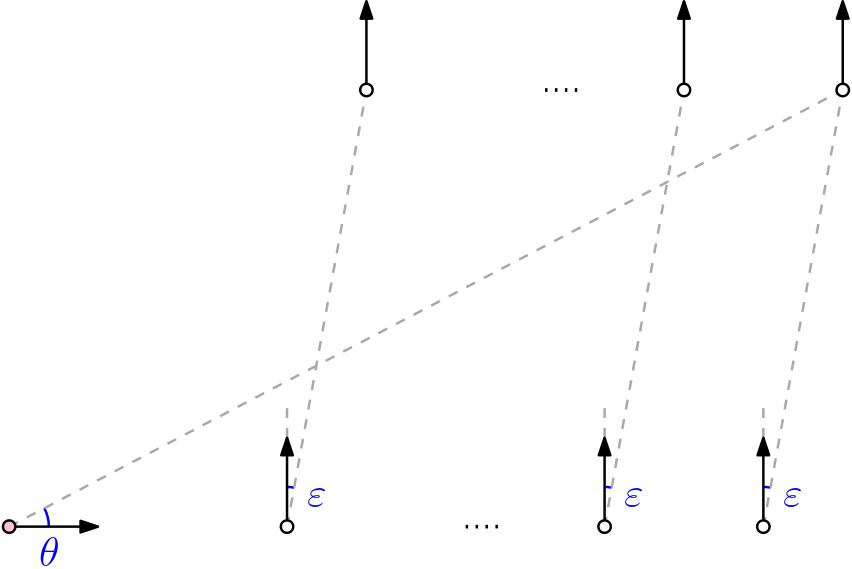
\includegraphics[height=5cm]{AFTP/makespan.png}
  \end{minipage}

  \bigbreak
  \only<2,3>{Seja $\mathbf{S}$ uma solução tal que $\mathbf{M}$ \textbf{é minimizada}.}
  \bigbreak
  \only<3>{Então, $M(S) = \varepsilon$ e $E(S) = \frac{n-1}{2} \cdot \varepsilon = O(n \cdot M(S))$.}
\end{frame}

%------------------------------------------------------------------------------%

\begin{frame}{Resultados Anteriores}
  \begin{thm}[Fekete e Krupke~\cite{Fe18}]
    Existe uma $9$-aproximação para o AFTP em 2D, assumindo um limite inferior de $\delta>0$ para a rotação inicial de qualquer satélite que mova sua antena.
  \end{thm}

  \pause
  \setbeamercolor{block body}{bg=red!20!white}
  \begin{thm}[Fekete e Krupke~\cite{Fe18}]
    É NP-difícil aproximar o AFTP em 2D dentro de um fator menor que $\nicefrac{5}{3}$.
  \end{thm}
\end{frame}


\section{Nossos Resultados}
\begin{frame}{Enunciados}
  \setbeamercolor{block body}{bg=seagreen!20!white}
  \begin{thm}
    Seja $\mathbf{I}$ uma instância do AFTP, $\mathbf{E}$ um número real e $\mathbf{k}$ um inteiro positivo.
    \pause

    Então, existe um algoritmo que roda em tempo ${(n\frac{Ek}{\delta})^{O(\frac{Ek}{\delta})}}$ e \pause ou prova que toda solução ótima requer mais de $\mathbf{E}$ de energia total\pause, ou encontra uma solução com \emph{makespan} no máximo ${(1+\nicefrac{1}{k}) \cdot \opt(I)}$.
  \end{thm}

  \pause

  \begin{thm}
    Para todo inteiro positivo $k$, existe uma \mbox{$(1+\nicefrac{1}{k})$-aproximação} para o E-AFTP, que roda em tempo \mbox{$(n\frac{k}{\delta})^{O(\frac{k}{\delta})}$}.
  \end{thm}
\end{frame}

\begin{frame}{Preparação}
  \centering
  Seja $\mu=\frac{\delta}{4k}$:
  \pause
  \begin{itemize}[<+->]
    \item Uma sequência é \textbf{$\mathbf{\mu}$-discreta} se todos os seus valores são múltiplos de $\mu$;

    \item Uma solução é \textbf{$\mathbf{\mu}$-discreta} se todos as suas sequências são $\mu$-discretas.
  \end{itemize}
\end{frame}

\begin{frame}{Lema Principal}
  \begin{lemma}[Silva \cite{Lu25}]
    Toda \textbf{solução racional} $S$ para $I$ pode ser convertida em uma solução $\mu$-discreta $S^\mu$ tal que \pause $M(S^\mu) \leq \left(1 + \frac{1}{k} \right) \cdot M(S)$ e $E(S^\mu) \leq \left(1 + \frac{1}{k} \right) \cdot E(S)$.
  \end{lemma}
\end{frame}

\begin{frame}{Ideia da Prova}
  \begin{minipage}{\linewidth}
    \centering
    \only<1>{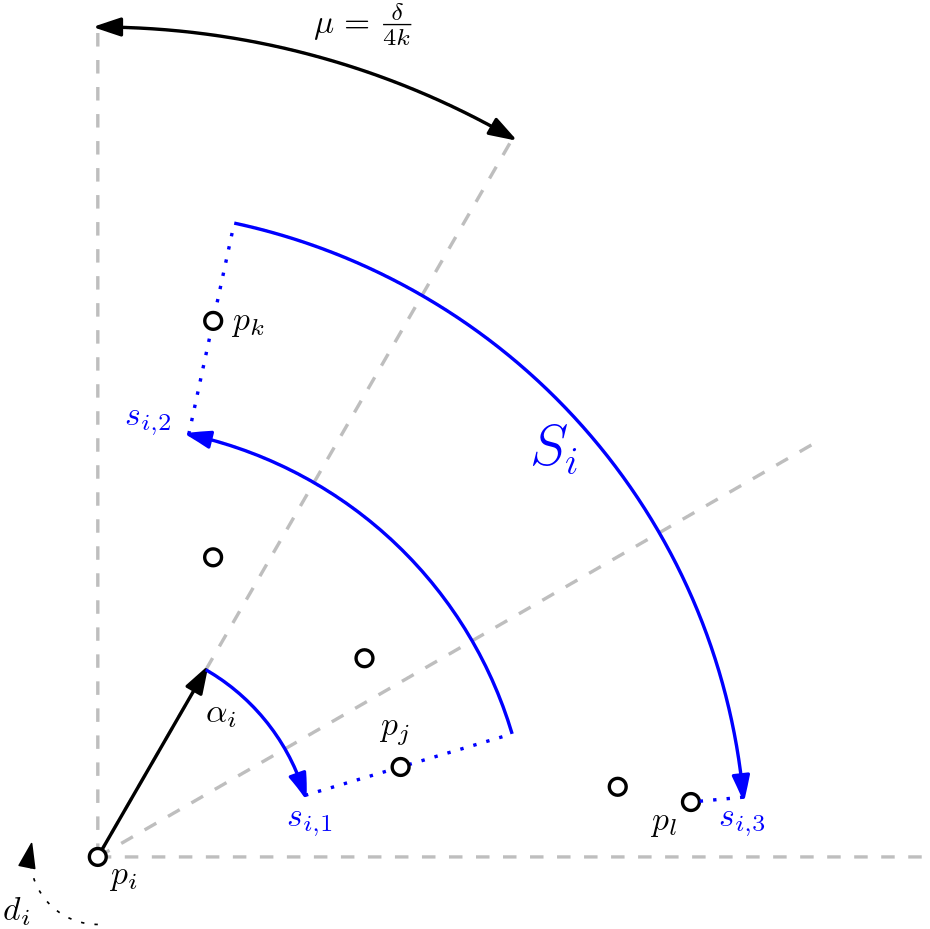
\includegraphics[height=7cm]{AFTP/algo1.png}}
    \only<2>{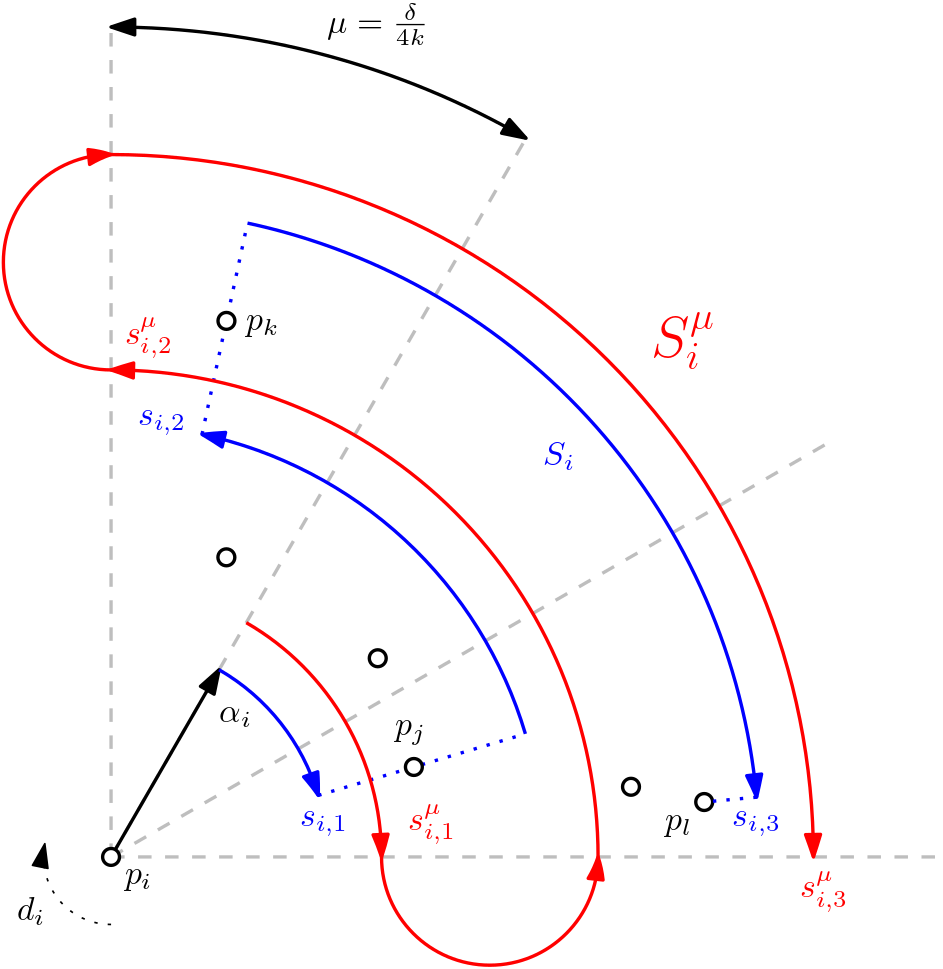
\includegraphics[height=7cm]{AFTP/algo2.png}}
  \end{minipage}
\end{frame}

\begin{frame}{Usando o Lema}
    Consideramos apenas soluções $\mu$-discretas cuja energia total não excede $(1 + \nicefrac{1}{k}) \cdot E$!
\end{frame}

\begin{frame}{Conclusão}
  \begin{itemize}[<+->]
    \item Após cada rotação, a antena de um satélite estará em uma das $O\left( \nicefrac{E}{\mu} \right)$ \textbf{orientações possíveis};

    \item Existem $O\left( \nicefrac{E^2}{\mu^2} \right)$ \textbf{transições válidas} por satélite, totalizando $O\left( n \cdot \nicefrac{E^2}{\mu^2} \right)$ transições;

    \item Apenas $O\left( \nicefrac{E}{\mu} \right)$ delas podem ser selecionadas;

    \bigbreak
    \item Total de $\binom{O\left( n \cdot \nicefrac{E^2}{\mu^2} \right)}{O\left( \nicefrac{E}{\mu} \right)}$ \textbf{soluções possíveis}, que podem ser checadas em tempo $\left( n \frac{E k}{\delta} \right)^{O\left( \nicefrac{E k}{\delta} \right)}$.
  \end{itemize}
\end{frame}


\section{Trabalhos Futuros}
\begin{frame}{Problemas em Aberto}
  \begin{itemize}[<+->]
    \item Tempo de execução $f(E, k, \delta) \cdot n ^ {O(1)}$ (\textbf{FPT}) ao invés de $g(E, k, \delta) \cdot n ^ {h(E, k, \delta)}$ (\textbf{XP});

    \item Dificuldade do E-AFTP;

    \item Resultados para 3D.
  \end{itemize}
\end{frame}


\begin{frame}[plain,noframenumbering]
  \large{\centerline{Obrigado a todos pela atenção...}}
  \pause
  \Huge{\centerline{Fim.}}
\end{frame}

%-----------------------[ Bibliography ]---------------------------------------%

\appendix

\setbeamertemplate{bibliography item}[text]
\begin{frame}
  \frametitle{Referências}
  {
    \tiny
    \bibliographystyle{alpha}
    \bibliography{bibliography}
  }
\end{frame}

%-----------------------[ Backup ]---------------------------------------------%


\end{document}
